\documentclass[12pt,a4paper]{article}

% ─── Page Layout ───────────────────────────────────────────────────────────────
\usepackage[a4paper, margin=0.8in, headheight=14pt]{geometry}

% ─── Fonts (XeLaTeX) ───────────────────────────────────────────────────────────
\usepackage{fontspec}
\usepackage{unicode-math}
\setmainfont{TeX Gyre Pagella}
\setmonofont[Scale=0.88]{TeX Gyre Cursor}
\setmathfont{Latin Modern Math}

% ─── Packages ──────────────────────────────────────────────────────────────────
\usepackage{xcolor}
\usepackage{colortbl}
\usepackage{titlesec}
\usepackage{enumitem}
\usepackage{tabularx}
\usepackage{booktabs}
\usepackage{array}
\usepackage{amsmath}
\usepackage{tikz}
\usetikzlibrary{shapes.geometric, arrows.meta, positioning, calc, fit, decorations.pathreplacing}
\usepackage{tcolorbox}
\tcbuselibrary{skins, breakable}
\usepackage{hyperref}
\usepackage{fancyhdr}
\usepackage{graphicx}
\usepackage{microtype}
\hyphenpenalty=10000
\exhyphenpenalty=10000
\sloppy
\usepackage{caption}
\usepackage{setspace}
\usepackage{multirow}
\usepackage{tocloft}

% ─── Q&A helper ────────────────────────────────────────────────────────────────
\newcommand{\Q}[1]{\textbf{#1}\par\noindent\ignorespaces}

% ─── Colour Palette ────────────────────────────────────────────────────────────
\definecolor{myred}{RGB}{196,30,58}
\definecolor{mydark}{RGB}{30,30,50}
\definecolor{mygreen}{RGB}{14,120,80}
\definecolor{myteal}{RGB}{0,130,140}
\definecolor{myamber}{RGB}{180,100,0}
\definecolor{mypurple}{RGB}{100,30,160}
\definecolor{mygray}{RGB}{246,247,249}
\definecolor{mgframe}{RGB}{180,185,200}
\definecolor{watermark}{RGB}{145,150,170}
\definecolor{hdrred}{RGB}{250,232,235}
\definecolor{hdrgreen}{RGB}{220,244,233}
\definecolor{hdrteal}{RGB}{220,242,244}
\definecolor{hdramber}{RGB}{253,242,215}
\definecolor{hdrpurple}{RGB}{238,228,255}

% ─── Section Formatting ────────────────────────────────────────────────────────
\titleformat{\section}
  {\large\bfseries\color{myred}}{\thesection.}{0.5em}{}
  [\vspace{1pt}{\color{myred}\rule{\linewidth}{0.8pt}}]
\titleformat{\subsection}
  {\normalsize\bfseries\color{myteal}}{\thesubsection}{0.5em}{}
\titlespacing*{\section}{0pt}{18pt}{7pt}
\titlespacing*{\subsection}{0pt}{11pt}{4pt}

% ─── Paragraph ─────────────────────────────────────────────────────────────────
\setlength{\parindent}{0pt}
\setlength{\parskip}{4pt}

% ─── TOC Styling ───────────────────────────────────────────────────────────────
\renewcommand{\cfttoctitlefont}{\large\bfseries\color{myred}}
\renewcommand{\cftaftertoctitle}{\par\noindent{\color{myred}\rule{\linewidth}{0.8pt}}}
\setlength{\cftbeforetoctitleskip}{0pt}
\setlength{\cftaftertoctitleskip}{6pt}
\renewcommand{\cftsecfont}{\normalsize\bfseries\color{mydark}}
\renewcommand{\cftsecpagefont}{\normalsize\bfseries\color{mydark}}
\renewcommand{\cftsecleader}{\cftdotfill{\cftdotsep}}
\setlength{\cftbeforesecskip}{7pt}
\renewcommand{\cftsubsecfont}{\small\color{mydark}}
\renewcommand{\cftsubsecpagefont}{\small\color{mydark}}
\setlength{\cftbeforesubsecskip}{3pt}
\setlength{\cftsubsecindent}{1.4em}

% ─── Table helpers ─────────────────────────────────────────────────────────────
\renewcommand{\arraystretch}{1.45}
\setlength{\tabcolsep}{6pt}
\arrayrulecolor{mydark}
\newcolumntype{B}[1]{>{\small\bfseries\raggedright\arraybackslash}m{#1}}
\newcolumntype{Y}{>{\small\raggedright\arraybackslash}X}
\renewcommand{\tabularxcolumn}[1]{m{#1}}

% ─── Header / Footer ───────────────────────────────────────────────────────────
\pagestyle{fancy}
\fancyhf{}
\fancyhead[L]{\small\color{myred}\textbf{PE-EC801C}\;\color{mydark}--- Error Correcting Codes}
\fancyhead[R]{\small\color{myteal}\textbf{Module 2 Notes}}
\fancyfoot[C]{\small\color{mydark}\thepage}
\fancyfoot[R]{\small\color{watermark}\textit{\copyright\ Biraj}}
\renewcommand{\headrulewidth}{0.5pt}
\renewcommand{\footrulewidth}{0.3pt}

% ─── Hyperref ──────────────────────────────────────────────────────────────────
\hypersetup{
  colorlinks=true, linkcolor=myteal, urlcolor=myteal,
  pdfauthor={Biraj Sarkar},
  pdftitle={PE-EC801C --- Module 2 Notes}
}

% ─── tcolorbox styles ──────────────────────────────────────────────────────────
\tcbset{
  tikzbox/.style={
    colback=mygray, colframe=mgframe, boxrule=0.6pt, arc=4pt,
    left=8pt, right=8pt, top=6pt, bottom=6pt,
    colbacktitle=mgframe, coltitle=mydark,
    fonttitle=\small\bfseries
  },
  defbox/.style={
    colback=hdrgreen, colframe=mygreen, boxrule=0.8pt, arc=4pt,
    left=9pt, right=9pt, top=6pt, bottom=6pt,
    colbacktitle=mygreen, coltitle=white,
    fonttitle=\small\bfseries
  },
  formulabox/.style={
    colback=hdrteal, colframe=myteal, boxrule=0.8pt, arc=4pt,
    left=9pt, right=9pt, top=7pt, bottom=7pt,
    colbacktitle=myteal, coltitle=white,
    fonttitle=\small\bfseries
  },
  examplebox/.style={
    colback=hdramber, colframe=myamber, boxrule=0.8pt, arc=4pt,
    left=9pt, right=9pt, top=6pt, bottom=6pt,
    colbacktitle=myamber, coltitle=white,
    fonttitle=\small\bfseries
  },
  masonbox/.style={
    colback=hdrpurple, colframe=mypurple, boxrule=0.8pt, arc=4pt,
    left=9pt, right=9pt, top=6pt, bottom=6pt,
    colbacktitle=mypurple, coltitle=white,
    fonttitle=\small\bfseries
  },
  exambox/.style={
    colback=hdrpurple, colframe=mypurple, boxrule=1pt, arc=5pt,
    left=10pt, right=10pt, top=8pt, bottom=8pt,
    colbacktitle=mypurple, coltitle=white,
    fonttitle=\bfseries,
    breakable, title after break={\textbf{Frequently Asked / Viva Questions (contd.)}}}
}
\tcbset{breakable}
\tcbset{after={\color{black}}}

% ─── TikZ styles ───────────────────────────────────────────────────────────────
\tikzset{
  reg/.style={rectangle, draw=myteal, fill=hdrteal,
    minimum width=0.85cm, minimum height=0.85cm, align=center,
    font=\small\bfseries, line width=0.7pt},
  adder/.style={circle, draw=myamber, fill=hdramber,
    minimum size=0.45cm, font=\small\bfseries, line width=0.8pt, inner sep=0pt},
  mult/.style={circle, draw=mypurple, fill=hdrpurple,
    minimum size=0.45cm, font=\small, line width=0.7pt, inner sep=0pt},
  arrow/.style={-Stealth, thick, color=mydark},
  line/.style={thick, color=mydark}
}

% ═══════════════════════════════════════════════════════════════════════════════
\begin{document}
% ═══════════════════════════════════════════════════════════════════════════════

\begin{center}
  {\LARGE\bfseries\color{myred} PE-EC801C --- Error Correcting Codes}\\[5pt]
  {\normalsize\color{mydark} Semester VIII \quad$\bullet$\quad 3L:0T:0P \quad$\bullet$\quad 3 Credits}\\[3pt]
  {\normalsize\color{myteal}\textbf{Module 2: Galois Fields and Cyclic Codes}}\\[3pt]
  {\small\color{mydark} CGEC \;$|$\; B.Tech ECE (2023--27) \;$|$\; \textit{Biraj Sarkar}}
\end{center}
\vspace{2pt}
\noindent{\color{myred}\rule{\linewidth}{1.5pt}}
\vspace{2pt}

\hypersetup{linkcolor=mydark}
\tableofcontents
\hypersetup{linkcolor=myteal}
\newpage

% ===============================================================================
\section{Algebraic Background --- Groups, Rings and Fields}
% ===============================================================================

To design and analyze cyclic, BCH, and Reed-Solomon codes, we must establish their underlying algebraic structures.

\begin{tcolorbox}[defbox, title={\textbf{Algebraic Structures Summary}}]
\begin{itemize}[leftmargin=*, itemsep=3pt, topsep=0pt]
  \item \textbf{Group:} A set $G$ with a binary operation $*$ satisfying: closure ($a * b \in G$), associativity ($a * (b * c) = (a * b) * c$), existence of identity $e$ ($a * e = a$), and existence of inverse $a^{-1}$ ($a * a^{-1} = e$). If $a * b = b * a$, it is an \textbf{Abelian Group}.
  \item \textbf{Ring:} A set $R$ with two binary operations (addition $+$ and multiplication $\cdot$) where $(R, +)$ is an Abelian group, multiplication is associative and distributive over addition, and contains a multiplicative identity $1$.
  \item \textbf{Field:} A ring $F$ where multiplication is commutative, and every non-zero element $a \in F$ has a multiplicative inverse $a^{-1}$ such that $a \cdot a^{-1} = 1$.
\end{itemize}
\end{tcolorbox}

\subsection{Finite Fields (Galois Fields)}
A field containing a finite number of elements is a \textbf{Galois Field}, denoted as $\text{GF}(q)$. A finite field exists if and only if $q$ is a prime power: $q = p^m$, where $p$ is a prime number (called the \textbf{characteristic} of the field) and $m$ is a positive integer.
\begin{itemize}[leftmargin=*, itemsep=2pt]
  \item For $m=1$, $\text{GF}(p)$ is the prime field consisting of integers $\{0, 1, \dots, p-1\}$ under modulo-$p$ arithmetic.
  \item For $m > 1$, $\text{GF}(2^m)$ is an extension field constructed using polynomials.
\end{itemize}

\subsection{Extension Field Construction}
To construct $\text{GF}(2^m)$, we choose an \textbf{irreducible polynomial} $p(x)$ (a polynomial that cannot be factored into lower-degree polynomials over $\text{GF}(2)$) of degree $m$. Let $\alpha$ be a root of $p(x)$, such that $p(\alpha) = 0$.
The elements of $\text{GF}(2^m)$ can be represented in three ways:
1. \textbf{Power representation:} $\{0, \alpha^0, \alpha^1, \dots, \alpha^{2^m-2}\}$.
2. \textbf{Polynomial representation:} Binary combinations of $\{1, \alpha, \alpha^2, \dots, \alpha^{m-1}\}$.
3. \textbf{Vector representation:} Binary coefficients of the polynomial representation.

\begin{tcolorbox}[examplebox, title={\textbf{Construction of GF($2^3$) using $p(x) = x^3 + x + 1$}}]
Let $\alpha$ be a root of $p(x) = x^3 + x + 1$, which satisfies $p(\alpha) = 0$:\par
\[
\alpha^3 \oplus \alpha \oplus 1 = 0 \implies \alpha^3 = \alpha \oplus 1
\]
The $2^3 = 8$ elements of $\text{GF}(8)$ are:
\par\noindent
\renewcommand{\arraystretch}{1.2}
\begin{tabularx}{\linewidth}{|>{\centering\arraybackslash}X|>{\centering\arraybackslash}X|>{\centering\arraybackslash}X|}
\hline
\textbf{Power Form} & \textbf{Polynomial Form} & \textbf{Vector Form $(a_2, a_1, a_0)$} \\
\hline
$0$ & $0$ & $(0, 0, 0)$ \\
\hline
$\alpha^0$ & $1$ & $(0, 0, 1)$ \\
\hline
$\alpha^1$ & $\alpha$ & $(0, 1, 0)$ \\
\hline
$\alpha^2$ & $\alpha^2$ & $(1, 0, 0)$ \\
\hline
$\alpha^3$ & $\alpha \oplus 1$ & $(0, 1, 1)$ \\
\hline
$\alpha^4$ & $\alpha^2 \oplus \alpha$ & $(1, 1, 0)$ \\
\hline
$\alpha^5$ & $\alpha^2 \oplus \alpha \oplus 1$ & $(1, 1, 1)$ \\
\hline
$\alpha^6$ & $\alpha^2 \oplus 1$ & $(1, 0, 1)$ \\
\hline
\end{tabularx}
\end{tcolorbox}

\subsection{Primitive Elements and Minimal Polynomials}
\begin{itemize}[leftmargin=*, itemsep=3pt]
  \item \textbf{Primitive Element:} An element $\beta \in \text{GF}(2^m)$ whose successive powers generate all $2^m-1$ non-zero elements of the field.
  \item \textbf{Conjugate Elements:} If $\beta \in \text{GF}(2^m)$, its conjugates over $\text{GF}(2)$ are:
    \[ \beta, \beta^2, \beta^{2^2}, \dots, \beta^{2^{d-1}} \]
    where $d$ is the smallest integer such that $\beta^{2^d} = \beta$.
  \item \textbf{Minimal Polynomial ($m(x)$):} The lowest-degree polynomial with binary coefficients that has $\beta$ (and its conjugates) as a root:
    \[ m(x) = \prod_{i=0}^{d-1} (x - \beta^{2^i}) \]
\end{itemize}

% ===============================================================================
\section{Factorization of \texorpdfstring{$X^n - 1$}{X^n - 1} over a Finite Field}
% ===============================================================================

Let $n$ be the block length of a cyclic code. The polynomial $X^n \oplus 1$ can be factored into a product of irreducible polynomials over $\text{GF}(2)$:
\[ X^n \oplus 1 = f_1(x) f_2(x) \dots f_r(x) \]
The roots of these irreducible factors are elements of $\text{GF}(2^m)$, where $m$ is the multiplicative order of $2$ modulo $n$.
Every irreducible factor $f_i(x)$ is the minimal polynomial of a root of $X^n \oplus 1$.

\begin{tcolorbox}[examplebox, title={\textbf{Factorization Example for $n=7$}}]
We wish to factor $X^7 \oplus 1$ over $\text{GF}(2)$.
The roots of $X^7 \oplus 1 = 0$ are the 7-th roots of unity in $\text{GF}(8)$, which are $\{1, \alpha, \alpha^2, \alpha^3, \alpha^4, \alpha^5, \alpha^6\}$.
Grouping roots into conjugate classes (cyclotomic cosets):
\begin{itemize}[leftmargin=*, itemsep=2pt]
  \item Coset 1: $\{1\}$ (minimal polynomial: $x \oplus 1$)
  \item Coset 2: $\{\alpha, \alpha^2, \alpha^4\}$ (minimal polynomial: $x^3 \oplus x \oplus 1$)
  \item Coset 3: $\{\alpha^3, \alpha^6, \alpha^5\}$ (minimal polynomial: $x^3 \oplus x^2 \oplus 1$)
\end{itemize}
Therefore, the factorization of $X^7 \oplus 1$ over $\text{GF}(2)$ is:
\[ X^7 \oplus 1 = (x \oplus 1)(x^3 \oplus x \oplus 1)(x^3 \oplus x^2 \oplus 1) \]
\end{tcolorbox}

% ===============================================================================
\section{Cyclic Codes}
% ===============================================================================

A \textbf{cyclic code} is a linear block code where any cyclic shift of a codeword is also a valid codeword.

\begin{tcolorbox}[defbox, title={\textbf{Formal Cyclic Shift Property}}]
If $c = (c_0, c_1, \dots, c_{n-1}) \in C$ is a codeword, then its cyclic shift:
\[ c^{(1)} = (c_{n-1}, c_0, c_1, \dots, c_{n-2}) \in C \]
is also a valid codeword.
\end{tcolorbox}

\subsection{Polynomial Representation}
Codewords are represented as polynomials of degree at most $n-1$:
\[ c(x) = c_0 \oplus c_1 x \oplus c_2 x^2 \oplus \dots \oplus c_{n-1} x^{n-1} \]
A cyclic shift corresponds to multiplying $c(x)$ by $x$ modulo $X^n \oplus 1$:
\[ x \cdot c(x) \pmod{X^n \oplus 1} = c_{n-1} \oplus c_0 x \oplus c_1 x^2 \oplus \dots \oplus c_{n-2} x^{n-1} \]
Algebraically, a cyclic code of length $n$ is an \textbf{ideal} in the quotient polynomial ring $\text{GF}(2)[x] / (X^n \oplus 1)$.

\subsection{The Generator Polynomial \texorpdfstring{$g(x)$}{g(x)}}
A cyclic code is uniquely defined by a single generator polynomial $g(x)$.
\begin{tcolorbox}[defbox, title={\textbf{Properties of the Generator Polynomial}}]
\begin{itemize}[leftmargin=*, itemsep=3pt, topsep=0pt]
  \item $g(x)$ is the unique, monic polynomial of minimum degree in the code.
  \item The degree of $g(x)$ is equal to the number of parity check bits: $\deg(g(x)) = n - k$.
  \item $g(x)$ is a factor of $X^n \oplus 1$:
    \[ X^n \oplus 1 = g(x) \cdot h(x) \]
    where $h(x)$ is the \textbf{parity check polynomial} of degree $k$.
\end{itemize}
\end{tcolorbox}

Every codeword polynomial $c(x)$ in the code can be written as a product of a message polynomial $m(x)$ (of degree $< k$) and the generator polynomial $g(x)$:
\[ c(x) = m(x) \cdot g(x) \]

\subsection{Systematic Encoding Algorithm}
To construct a systematic cyclic code where the message bits occupy the higher-order coefficients of $c(x)$, we use the following steps:
\begin{tcolorbox}[formulabox, title={\textbf{Systematic Cyclic Encoding Steps}}]
\begin{enumerate}[label=\textbf{Step \arabic*:}, leftmargin=2.0cm, itemsep=2pt]
  \item Multiply the message polynomial $m(x)$ by $x^{n-k}$ to shift it into the systematic position.
  \item Divide $x^{n-k}m(x)$ by the generator polynomial $g(x)$ to find the remainder $d(x)$:
    \[ x^{n-k}m(x) = q(x)g(x) \oplus d(x) \]
    where $\deg(d(x)) < n-k$.
  \item Construct the codeword polynomial:
    \[ c(x) = x^{n-k}m(x) \oplus d(x) = q(x)g(x) \]
\end{enumerate}
\end{tcolorbox}

Since addition and subtraction are identical in binary (modulo-2), adding $d(x)$ to $x^{n-k}m(x)$ cancels the remainder, leaving a polynomial that is a multiple of $g(x)$ (hence a valid codeword).

% ===============================================================================
\section{Feedback Shift Register Encoders and Syndrome Calculators}
% ===============================================================================

The polynomial division needed for systematic cyclic encoding is implemented in hardware using a \textbf{Feedback Shift Register (FSR)}.

\subsection{Systematic FSR Encoder Circuit}
Let $g(x) = g_0 \oplus g_1 x \oplus \dots \oplus g_{n-k-1} x^{n-k-1} \oplus x^{n-k}$ be the generator polynomial. The shift register consists of $n-k$ stages.

\begin{tcolorbox}[tikzbox, title={Systematic Cyclic Encoder Circuit}]
\centering
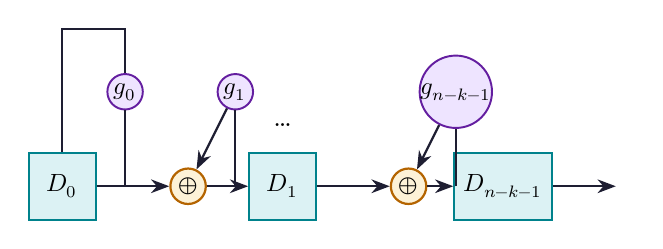
\begin{tikzpicture}[node distance=1.2cm]
  \node[reg] (r0) at (0,0) {$D_0$};
  \node[adder] (a1) at (1.6,0) {$\oplus$};
  \node[reg] (r1) at (2.8,0) {$D_1$};
  \node[adder] (a2) at (4.4,0) {$\oplus$};
  \node[reg] (r2) at (5.6,0) {$D_{n-k-1}$};

  \draw[arrow] (r0) -- (a1);
  \draw[arrow] (a1) -- (r1);
  \draw[arrow] (r1) -- (a2);
  \draw[arrow] (a2) -- (r2);

  \node[mult] (m0) at (0.8, 1.2) {$g_0$};
  \node[mult] (m1) at (2.2, 1.2) {$g_1$};
  \node[mult] (m2) at (5.0, 1.2) {$g_{n-k-1}$};

  \draw[line] (0.8, 0) -- (m0);
  \draw[line] (m0) |- (0, 2.0) -- (r0);
  
  \draw[line] (2.2, 0) -- (m1);
  \draw[arrow] (m1) -- (a1);

  \draw[line] (5.0, 0) -- (m2);
  \draw[arrow] (m2) -- (a2);
  
  \node[right=0.8cm of r2] (out) {};
  \draw[arrow] (r2) -- (out);
  
  \node[above=0.2cm of r1] {\dots};
\end{tikzpicture}
\end{tcolorbox}

The division operates as follows:
\begin{enumerate}[leftmargin=*, itemsep=3pt]
  \item The gate switch is closed. The $k$ message bits are fed into the channel and the feedback path simultaneously.
  \item After $k$ clock cycles, the shift registers contain the remainder coefficients (parity bits).
  \item The gate switch is opened, disabling feedback, and the parity bits are shifted out to complete the $n$-bit systematic codeword.
\end{enumerate}

\subsection{FSR Syndrome Calculator Circuit}
The syndrome $S(x)$ of a received polynomial $r(x)$ is the remainder of $r(x)$ divided by $g(x)$:
\[ S(x) = r(x) \pmod{g(x)} \]
This is implemented using a feedback shift register similar to the encoder.

\begin{tcolorbox}[tikzbox, title={Syndrome Calculator Circuit}]
\centering
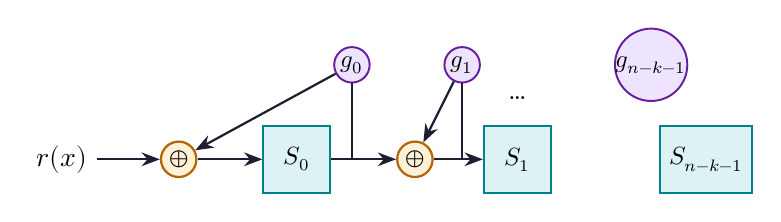
\begin{tikzpicture}[node distance=1.2cm]
  \node[adder] (inadd) at (-1.5, 0) {$\oplus$};
  \node[reg] (s0) at (0,0) {$S_0$};
  \node[adder] (sadd1) at (1.5,0) {$\oplus$};
  \node[reg] (s1) at (2.8,0) {$S_1$};
  \node[reg] (s2) at (5.2,0) {$S_{n-k-1}$};

  \draw[arrow] (inadd) -- (s0);
  \draw[arrow] (s0) -- (sadd1);
  \draw[arrow] (sadd1) -- (s1);
  
  \node[mult] (g0) at (0.7, 1.2) {$g_0$};
  \node[mult] (g1) at (2.1, 1.2) {$g_1$};
  \node[mult] (g2) at (4.5, 1.2) {$g_{n-k-1}$};

  \draw[line] (0.7, 0) -- (g0);
  \draw[arrow] (g0) -- (inadd);
  
  \draw[line] (2.1, 0) -- (g1);
  \draw[arrow] (g1) -- (sadd1);
  
  \node[left=0.8cm of inadd] (rx) {$r(x)$};
  \draw[arrow] (rx) -- (inadd);
  
  \node[above=0.2cm of s1] {\dots};
\end{tikzpicture}
\tcbset{after={\color{black}}}
\end{tcolorbox}

% ===============================================================================
\section{Spectral Properties of Cyclic Codes}
% ===============================================================================

Like time-domain signals, codewords of cyclic codes have equivalent frequency-domain descriptions using the \textbf{Discrete Fourier Transform (DFT)} over finite fields.
Let $v = (v_0, v_1, \dots, v_{n-1})$ be a vector over $\text{GF}(2^m)$ where $n$ divides $2^m - 1$. Let $\alpha$ be a primitive $n$-th root of unity in $\text{GF}(2^m)$.

\begin{tcolorbox}[defbox, title={\textbf{Finite Field Discrete Fourier Transform}}]
The DFT of $v$, denoted $V = (V_0, V_1, \dots, V_{n-1})$, consists of elements in $\text{GF}(2^m)$ computed by:
\[ V_j = \sum_{i=0}^{n-1} v_i \alpha^{ij}, \quad j = 0, 1, \dots, n-1 \]
The inverse DFT is:
\[ v_i = \sum_{j=0}^{n-1} V_j \alpha^{-ij}, \quad i = 0, 1, \dots, n-1 \]
\end{tcolorbox}

\subsection{Spectral Constraints and Ideals}
The cyclic shift of a vector $v$ in the time domain corresponds to multiplying its spectral components by powers of $\alpha$:
\[ v^{(1)} \longleftrightarrow (\alpha^0 V_0, \alpha^1 V_1, \dots, \alpha^{n-1} V_{n-1}) \]
Therefore, a cyclic code can be defined in the spectral domain by forcing certain spectral components to zero:
\[ C = \{ c \in \text{GF}(2)^n \mid C_j = 0 \text{ for all } j \in \mathcal{K} \} \]
where $\mathcal{K}$ is a set of spectral indices. This spectral property is the foundation for designing BCH and Reed-Solomon codes.

% ═══════════════════════════════════════════════════════════════════════════════
% QUICK REVISION PAGE
% ═══════════════════════════════════════════════════════════════════════════════
\newpage
\begin{center}
  {\large\bfseries\color{myred} Quick Revision --- Module 2}\\[3pt]
  {\small\color{mydark} Galois Fields \& Cyclic Codes $|$ PE-EC801C}
\end{center}
\noindent{\color{myred}\rule{\linewidth}{1.2pt}}
\vspace{4pt}

\begin{tcolorbox}[formulabox, title={\textbf{Key Formulas and Metrics at a Glance}}]
\renewcommand{\arraystretch}{1.35}
\begin{tabularx}{\linewidth}{B{5.0cm} X}
Galois Field order & $q = p^m$ ($p$ is prime characteristic) \\[4pt]
Roots of Unity factor & $X^n \oplus 1 = g(x) \cdot h(x)$ \\[4pt]
Generator degree & $\deg(g(x)) = n - k$ \\[4pt]
Systematic Codeword polynomial & $c(x) = x^{n-k}m(x) \oplus [x^{n-k}m(x) \pmod{g(x)}]$ \\[4pt]
Modulo-2 addition relation & $a(x) \oplus b(x) = a(x) - b(x)$ \\[4pt]
Parity relation & $g(x) \cdot h(x) \equiv 0 \pmod{X^n \oplus 1}$ \\[4pt]
Finite Field DFT spectrum & $V_j = \sum_{i=0}^{n-1} v_i \alpha^{ij}$ \\[4pt]
Conjugate elements of $\beta$ & $\beta^{2^0}, \beta^{2^1}, \beta^{2^2}, \dots, \beta^{2^{d-1}}$ \\[4pt]
Generator matrix polynomial & $G = \begin{bmatrix} g(x) \\ x g(x) \\ \vdots \\ x^{k-1}g(x) \end{bmatrix}$ in non-systematic form
\end{tabularx}
\end{tcolorbox}

\vspace{6pt}

\begin{tcolorbox}[defbox, title={\textbf{One-Line Definitions}}]
\begin{itemize}[leftmargin=*, itemsep=3pt, topsep=0pt]
  \item \textbf{Abelian Group:} A group where the binary operation is commutative ($a * b = b * a$).
  \item \textbf{Field:} An algebraic ring where multiplication is commutative and every non-zero element has a multiplicative inverse.
  \item \textbf{Galois Field:} A finite field containing a prime-power number of elements, denoted $\text{GF}(p^m)$.
  \item \textbf{Irreducible Polynomial:} A polynomial that cannot be factored into polynomials of lower degree over the same field.
  \item \textbf{Primitive Element:} An element whose powers generate all non-zero elements of a finite field.
  \item \textbf{Minimal Polynomial:} The lowest-degree binary polynomial having a field element (and its conjugates) as roots.
  \item \textbf{Cyclic Code:} A linear code where a cyclic shift of any codeword produces another valid codeword.
  \item \textbf{Generator Polynomial ($g(x)$):} The unique lowest-degree polynomial of a cyclic code, which divides $X^n \oplus 1$.
\end{itemize}
\end{tcolorbox}

\newpage

\begin{tcolorbox}[exambox, title={\textbf{Frequently Asked / Viva Questions}}]
\begin{enumerate}[topsep=0pt, label=\textbf{Q\arabic*.}, itemsep=5pt]
  \item \Q{What are the differences between groups, rings, and fields?}
    A group has one operation ($+$). A ring has two operations ($+$ and $\cdot$) and is an Abelian group under addition. A field is a commutative ring with a multiplicative identity where every non-zero element has a unique multiplicative inverse.
  \item \Q{Why do Galois Fields only exist for prime-power sizes $p^m$?}
    For fields of size $q$, the characteristic must be a prime $p$. The field forms a vector space over its prime subfield $\text{GF}(p)$ of dimension $m$. Therefore, the number of elements in the field is $p \times p \times \dots \times p = p^m$.
  \item \Q{How is systematic cyclic encoding performed algebraically?}
    First, the message $m(x)$ is multiplied by $x^{n-k}$ to shift it. Then, we find the remainder $d(x)$ of $x^{n-k}m(x)$ divided by $g(x)$. The systematic codeword polynomial is constructed as $c(x) = x^{n-k}m(x) \oplus d(x)$.
  \item \Q{Why must the generator polynomial $g(x)$ divide $X^n \oplus 1$?}
    A cyclic code of length $n$ is an ideal in the polynomial ring modulo $X^n \oplus 1$. The ideal is generated by $g(x)$. Since the identity codeword $0 \equiv X^n \oplus 1 \pmod{X^n \oplus 1}$ must be a multiple of $g(x)$, $g(x)$ must divide $X^n \oplus 1$.
  \item \Q{Explain how a feedback shift register circuit performs polynomial division.}
    FSRs use shift register stages as memory and XOR gates as modulo-2 adders. Feedback paths multiply register states by coefficients $g_i$. Feeding coefficients through the loop matches polynomial long division.
  \item \Q{What are conjugate elements in a finite field?}
    For an element $\beta \in \text{GF}(2^m)$, its conjugates over $\text{GF}(2)$ are its repeated squarings: $\{\beta, \beta^2, \beta^4, \dots, \beta^{2^{d-1}}\}$, where $d$ is the cycle length. They share the same minimal polynomial.
  \item \Q{What is the parity check polynomial $h(x)$ of a cyclic code?}
    The parity check polynomial is defined by $h(x) = (X^n \oplus 1) / g(x)$. It has degree $k$ and satisfies $c(x) \cdot h(x) \equiv 0 \pmod{X^n \oplus 1}$ for any codeword $c(x)$.
  \item \Q{What are the advantages of cyclic codes over general linear block codes?}
    Cyclic codes have rich algebraic properties allowing systematic design (like BCH codes). In hardware, encoding and syndrome calculations are implemented using simple feedback shift registers.
  \item \Q{What is a primitive polynomial?}
    A primitive polynomial of degree $m$ is an irreducible polynomial over $\text{GF}(2)$ that has a primitive element of $\text{GF}(2^m)$ as a root. Its roots generate the entire multiplicative group.
  \item \Q{Explain the spectral definition of cyclic codes.}
    Using the DFT over finite fields, cyclic shifts correspond to multiplying spectral elements by powers of $\alpha$. A cyclic code is defined by forcing specific spectral elements of the codewords to zero.
\end{enumerate}
\tcbset{after={\color{black}}}
\end{tcolorbox}

\vspace{6pt}

\begin{tcolorbox}[tikzbox, title={\textbf{Comparison of Linear Block Codes and Cyclic Codes}}]
\renewcommand{\arraystretch}{1.45}
\begin{tabularx}{\linewidth}{|B{3.2cm}|Y|Y|}
\hline
\textbf{Property} & \textbf{Linear Block Codes} & \textbf{Cyclic Codes} \\
\hline
Mathematical Model & Vector Spaces over $\text{GF}(2)$ & Ideals in the ring $\text{GF}(2)[x]/(X^n \oplus 1)$ \\
\hline
Defining Matrices & Generator $G$ and Parity $H$ & Generator $g(x)$ and Parity $h(x)$ polynomials \\
\hline
Encoding Hardware & Matrix multiplication circuits & Feedback Shift Registers (FSR) \\
\hline
Error Correction & Systematic bounding & Rich algebraic code design (BCH/RS) \\
\hline
\end{tabularx}
\end{tcolorbox}

\end{document}
